\documentclass[a4paper,11pt]{article}

% ---- Paquetes de color y tipografía ----
\usepackage[spanish]{babel}
\usepackage[T1]{fontenc}
\usepackage[utf8]{inputenc}
\usepackage{microtype}
\usepackage{xcolor}
\definecolor{mirosado}{RGB}{255,182,193}
\definecolor{rosafuerte}{RGB}{246, 173, 198}

% Color favorito del usuario
\usepackage[hidelinks]{hyperref}

\usepackage{marginnote}

% ---- Fuentes ----
\renewcommand\familydefault{\sfdefault}
\usepackage{tgheros}
\usepackage[scale=0.85]{FiraMono}


% ---- Matemáticas y símbolos ----
\usepackage{amsmath,amssymb,amsthm,textcomp}
\usepackage{cleveref}
% ---- Gráficos y circuitos ----
\usepackage{graphicx}
\usepackage{tikz}
\usepackage{circuitikz}
\usepackage{float}

% ---- Listados de código ----
\usepackage{listings}
\definecolor{stringcolor}{RGB}{167,0,0}
\definecolor{keywordcolor}{RGB}{0,102,204}
\definecolor{commentcolor}{RGB}{128,128,128}
\lstdefinelanguage{Arduino}{
  language=C++,
  keywords={void,int,boolean,for,while,if,else,return,analogRead,Serial,begin,print,pinMode,digitalWrite,analogWrite,delay},
  sensitive=true,
  morecomment=[l]{//},
  morecomment=[s]{/*}{*/},
  morestring=[b]",
  keywordstyle=\color{keywordcolor}\bfseries,
  stringstyle=\color{stringcolor},
  commentstyle=\color{commentcolor}\itshape,
  basicstyle=\small\ttfamily,
  numbers=left,
  numberstyle=\tiny\color{commentcolor},
  stepnumber=1,
  breaklines=true,
  frame=single
}

% ---- Cajas pedagógicas ----
\usepackage{tcolorbox}
\tcbset{
  tip/.style={colback=mirosado!20,colframe=mirosado!75!black,fonttitle=\bfseries},
  warning/.style={colback=red!10,colframe=red!75!black,fonttitle=\bfseries}
}

% ---- Márgenes y encabezados ----
\usepackage{geometry}
\geometry{left=25mm,right=25mm,top=20mm,bottom=20mm}
\usepackage{fancyhdr}
\pagestyle{fancy}
\fancyhead{}
\fancyhead[L]{\small \leftmark}
\fancyhead[R]{\small Taller: Introducción a microcontroladores}
\cfoot{\thepage}
\renewcommand{\headrulewidth}{0.5pt}

\begin{document}

% ---- Sin sangría y espaciado ----
\setlength{\parindent}{0pt}
\linespread{1.15}

% ---- Portada personalizada ----
\begin{titlepage}
  \begin{minipage}{0.48\textwidth}
    \raggedright
    {\Large\textbf{Universidad de Concepci\'on}}\\[0.2cm]
    {\normalsize Facultad de Ingenier\'ia}\\
    {\normalsize Facultad de Ciencias F\'isicas y Matem\'aticas}\\
    {\normalsize Sociedad de Rob\'otica RAS IEEE UdeC}
  \end{minipage}
  \hfill
  \begin{minipage}{0.48\textwidth}
    \raggedleft
    \includegraphics[width=1.5cm]{img/logo_udec.png}
    \hspace{0.5cm}
    \includegraphics[width=3.5cm]{img/logo_ras.png}
  \end{minipage}

  \vspace*{8cm}
  \centering

  {\Huge\bfseries\color{rosafuerte} Taller B\'asico de Microcontroladores}\\[1.2cm]
  {\LARGE \textit{Introducci\'on a los Microcontroladores}}\\[2cm]

  \vfill

  {\textbf{16 de junio de 2025}}

  \vspace*{1.5cm}
  \begin{tikzpicture}
    \draw[fill=rosafuerte!20,draw=rosafuerte] (0,0) rectangle (10,0.5);
  \end{tikzpicture}
\end{titlepage}

\tableofcontents
\newpage

\section*{Objetivos del Taller}
\addcontentsline{toc}{section}{Objetivos del Taller}

\begin{itemize}
  \item Comprender la arquitectura y funcionamiento básico de un microcontrolador.
  \item Identificar las diferencias entre microcontroladores y microprocesadores.
  \item Familiarizarse con los principales bloques que conforman un microcontrolador: CPU, memorias, periféricos, etc.
  \item Conocer diferentes familias y plataformas, como Arduino, ESP32 y STM32.
  \item Aplicar buenas prácticas de programación, conexión y pruebas en el desarrollo con microcontroladores.
  \item Explorar proyectos motivadores que permitan aprender haciendo.
\end{itemize}
\section{Conceptos Fundamentales}

\subsection{Microcontrolador }
Es un circuito integrado programable que contiene, en un solo chip, todos los componentes necesarios para ejecutar tareas de control automático en sistemas embebidos. En términos simples, actúa como un pequeño computador autónomo diseñado para realizar funciones específicas en dispositivos electrónicos.
\begin{itemize}
  \item Un \textbf {sistema embebido} es una combinación de hardware y software que opera de forma autónoma, generalmente con recursos limitados, y está embebido (integrado) dentro de un producto o sistema mayor. Son generalmente no reconfigurables por el usuario final
  
\end{itemize}

\subsection{Microprocesador}

Es el núcleo de un sistema de cómputo de propósito general. Se trata de un chip electrónico que interpreta y ejecuta instrucciones, coordinando el funcionamiento de los demás componentes mediante buses de datos, direcciones y control.  Es el cerebro de los sistemas computacionales de propósito general. A diferencia de un microcontrolador, no tiene todo integrado, pero es mucho más potente y versátil, ideal para ejecutar múltiples programas y gestionar grandes volúmenes de datos.


\section{Diferencias entre Microprocesador y Microcontrolador}

Los microprocesadores y microcontroladores son unidades de procesamiento digital que comparten similitudes en su estructura fundamental, pero están diseñados para cumplir funciones distintas dentro de los sistemas electrónicos.

\bigskip

Un microprocesador es una unidad central de procesamiento diseñada para sistemas de propósito general, como computadoras. Requiere componentes externos (RAM, ROM, puertos, etc.) para funcionar, lo que lo hace más complejo, costoso y con mayor consumo energético, pero con alta capacidad de procesamiento.

\bigskip

En cambio, un microcontrolador es un chip todo-en-uno que integra CPU, memoria y periféricos. Está pensado para tareas específicas en sistemas embebidos, como electrodomésticos o dispositivos IoT (El Internet de las Cosas). Su bajo consumo, simplicidad y costo reducido lo hacen ideal para aplicaciones de control automático.

\bigskip

En resumen, mientras que el microprocesador es ideal para sistemas complejos y versátiles, el microcontrolador está diseñado para aplicaciones dedicadas y embebidas que requieren simplicidad, confiabilidad y eficiencia energética. De manera más gráfica se puede observar:

\subsection{Tabla comparativa:}


\begin{center}
\begin{tabular}{|l|l|l|}
\hline
\textbf{Caracter\'istica} & \textbf{Microprocesador} & \textbf{Microcontrolador} \\
\hline
Componentes integrados & Solo CPU & CPU + memoria + I/O + perif\'ericos \\
Uso & Computaci\'on general & Sistemas embebidos / control dedicado \\
Complejidad del sistema & Alta & Baja \\
Coste & Alto & Econ\'omico \\
Velocidad y potencia & Alta & Moderada \\
Consumo de energ\'ia & Alto & Bajo \\
\hline
\end{tabular}
\end{center}

\section{03. Arquitectura b\'asica de un Microcontrolador}

\subsection{CPU}
La Unidad Central de Procesamiento (CPU) ejecuta las instrucciones del programa, y se encarga de realizar operaciones aritm\'eticas, l\'ogicas y de control. Es el "cerebro" del microcontrolador.

\subsection{Memorias}
Un microcontrolador contiene distintos tipos de memoria:
\begin{itemize}
  \item \textit{ROM/FLASH}: Almacenamiento permanente del programa.
  \item \textit{RAM}: Memoria de acceso aleatorio para almacenamiento temporal de datos.
  \item \textit{EEPROM}: Memoria no vol\'atil programable, adecuada para guardar configuraciones o datos persistentes.
\end{itemize}

\subsection{Perif\'ericos de Entrada/Salida (I/O)}
Los pines de entrada/salida permiten que el microcontrolador se comunique con el mundo exterior, leyendo sensores o activando actuadores como luces y motores.

\subsection{Temporizadores y Contadores}
Componentes que permiten medir intervalos de tiempo, generar se\~nales de modulación por ancho de pulso (PWM) o contar eventos, esenciales en tareas de control y sincronizaci\'on.

\begin{tcolorbox}[tip,title=Tip rápido]
Antes de alimentar un circuito, revisa conexiones y polaridad con un multímetro. ¡Evita cortos!
\end{tcolorbox}

\subsection{Conversores A/D y D/A (ADC/DAC)}
Los conversores anal\'ogico/digital y digital/anal\'ogico permiten al microcontrolador interactuar con se\~nales del mundo real, convirti\'endolas entre formatos anal\'ogico y digital.

\subsection{Sistema de Interrupciones}
Permite que el microcontrolador interrumpa la ejecuci\'on normal del programa para atender eventos urgentes, como una se\~nal de un sensor o un cambio en una entrada.

\subsection{M\'odulos de Comunicaci\'on}
Facilitan la transmisi\'on y recepci\'on de datos mediante protocolos como UART, SPI, I2C, as\'i como conectividad inal\'ambrica (WiFi, Bluetooth, USB), seg\'un el modelo del microcontrolador.

\section{04. Tipos y Familias de Microcontroladores}

\subsection{AVR (Arduino – Atmel/Microchip)}
Microcontroladores de 8 bits basados en arquitectura RISC. Usan frecuencias de reloj de hasta 16 MHz. Programables en Arduino IDE, lenguaje C/C++ simplificado. Muy usados en educaci\'on y prototipado.

\begin{figure}[h]
  \centering
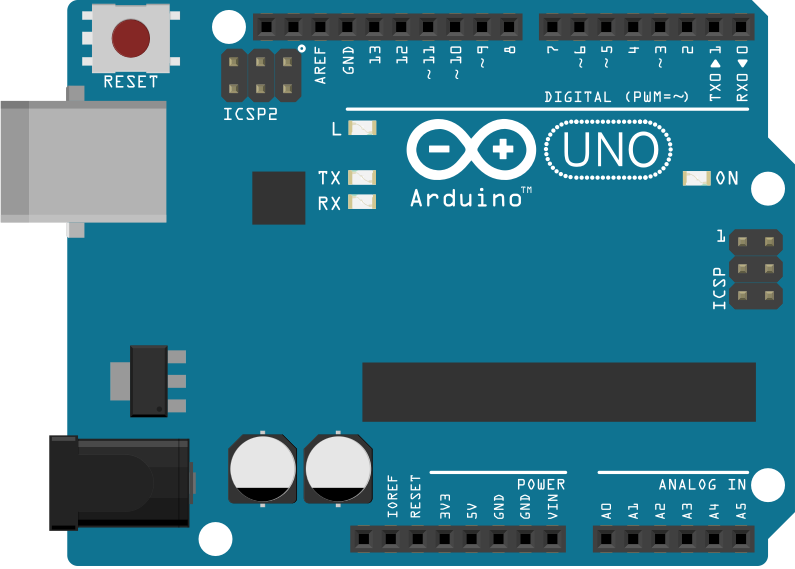
\includegraphics[width=0.5\textwidth]{img/ArduinoUNO.png}
  \caption{Placa Arduino Uno R3}
  \label{fig:uno}
\end{figure}


\subsection{ESP32 (Espressif Systems)}
Microcontrolador de 32 bits con WiFi y Bluetooth integrados. Doble n\'ucleo, hasta 240 MHz. Compatible con Arduino IDE, PlatformIO, MicroPython y ESP-IDF. Ideal para proyectos IoT.

\begin{figure}[H]
  \centering
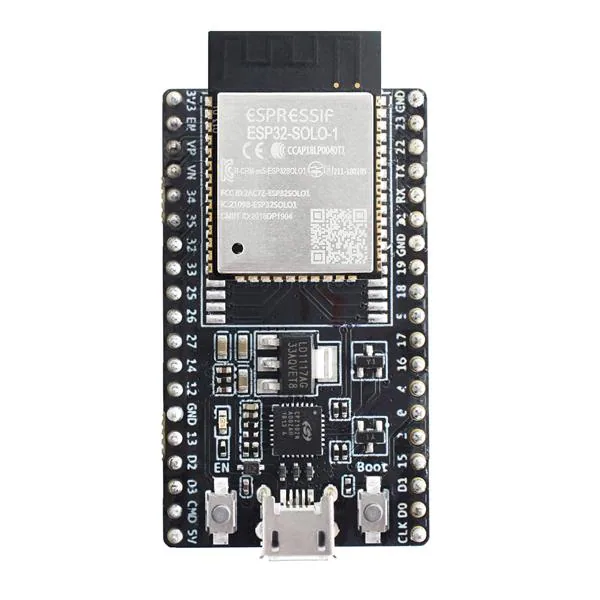
\includegraphics[width=0.3\textwidth]{img/ESP32.png}
  \caption{Placa ESP32}
  \label{fig:uno}
\end{figure}

\subsection{STM32 (STMicroelectronics)}
Familia de 32 bits basada en ARM Cortex-M. Potentes y eficientes energ\'eticamente, orientados a rob\'otica, procesamiento de se\~nales y dispositivos port\'atiles.

\begin{figure}[H]
  \centering
  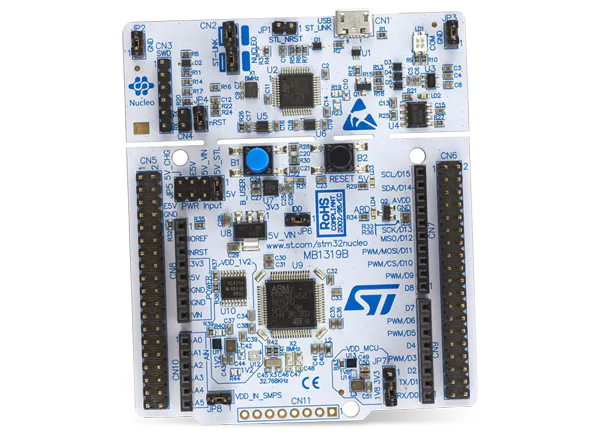
\includegraphics[width=0.3\textwidth]{img/STM32.png}
  \caption{Placa STM32}
  \label{fig:uno}
\end{figure}

\subsection{PIC (Microchip)}
Microcontroladores de 8 a 32 bits, robustos y confiables en la industria. Se programan en MPLAB X IDE, con control preciso de temporizadores y PWM.


\begin{figure}[H]
  \centering
  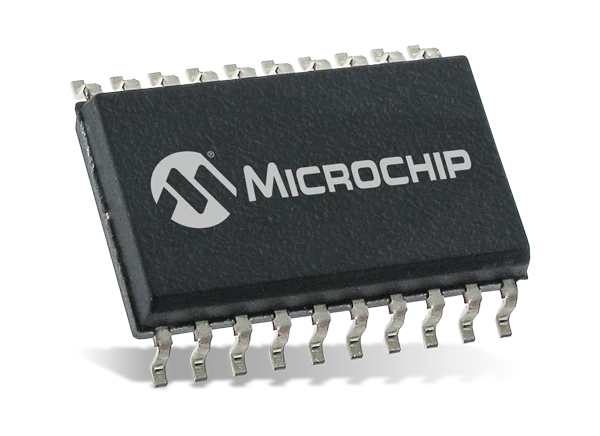
\includegraphics[width=0.3\textwidth]{img/PIC.png}
  \caption{Microchip}
  \label{fig:uno}
\end{figure}

\section{Buenas practicas}

\subsection{Lectura del Datasheet}
Antes de comenzar a trabajar con cualquier microcontrolador, es fundamental consultar su hoja de datos o \textit{datasheet}. Este documento proporciona informaci\'on detallada sobre las especificaciones el\'ectricas, caracter\'isticas de los pines, capacidades de memoria, m\'odulos disponibles (como timers, ADC, DAC, UART, etc.) y protocolos de comunicaci\'on soportados. Ignorar esta informaci\'on puede conducir a errores como alimentar el dispositivo con un voltaje incorrecto, configurar mal un pin o usar de forma inadecuada un perif\'erico.

Una buena pr\'actica es tener siempre el datasheet a mano durante el dise\~no del circuito y la programaci\'on. Adem\'as, muchas hojas de datos incluyen diagramas internos y secuencias de inicializaci\'on que permiten un mejor entendimiento del funcionamiento del chip.

\subsection{Configuraci\'on Correcta de Pines de Entrada y Salida}
Cada pin del microcontrolador puede actuar como entrada, salida digital, salida con modulación por ancho de pulso (PWM) o incluso como entrada anal\'ogica, dependiendo de su configuraci\'on. Es esencial definir correctamente el modo de cada pin antes de utilizarlo, ya que una configuraci\'on incorrecta puede generar lecturas err\'oneas, da\~nos en componentes conectados o fallos de funcionamiento.

Por ejemplo, si se configura un pin como salida y se conecta directamente a otro dispositivo que tambi\'en act\'ua como salida, podr\'ia producirse un cortocircuito. Por ello, debe utilizarse el bloque de configuraci\'on adecuado, como `pinMode()` en el entorno Arduino o registros de control en otros entornos.

\subsection{Protecci\'on contra Sobrecargas en Salidas Digitales}
Los pines de salida digital de un microcontrolador est\'an dise\~nados para entregar una corriente limitada, que normalmente est\'a entre 20 y 40 mA. Si se conecta una carga que requiere m\'as corriente, como un motor, un rel\'e o una tira LED, sin una interfaz adecuada, se puede da\~nar permanentemente el microcontrolador.

Para evitar esto, es recomendable emplear dispositivos de conmutaci\'on como transistores, MOSFETs o m\'odulos de drivers. Estos act\'uan como intermediarios, permitiendo al microcontrolador controlar grandes cargas sin exponerse directamente a altos niveles de corriente o tensiones externas.

\begin{tcolorbox}[tip,title=¡Atención!]
Nunca conectes directamente motores o cargas grandes al microcontrolador. ¡Usa transistores o relés!
\end{tcolorbox}

\subsection{Documentaci\'on Clara y Comentarios en el C\'odigo}
Un c\'odigo bien documentado no solo facilita el trabajo en equipo, sino que tambi\'en mejora la mantenibilidad del proyecto a lo largo del tiempo. Es muy com\'un que, tras semanas o meses, incluso el propio autor olvide la funci\'on de una secci\'on de c\'odigo mal comentada.

Algunas recomendaciones incluyen:
\begin{itemize}
  \item Utilizar nombres de variables descriptivos (por ejemplo, `temperaturaSensor` en lugar de `t`).
  \item Dividir el c\'odigo en funciones con tareas bien definidas.
  \item Agregar comentarios explicando el prop\'osito de bloques importantes.
  \item Especificar los rangos esperados para entradas y salidas.
\end{itemize}

Esto no solo ayuda a otros desarrolladores que revisen el c\'odigo, sino que tambi\'en es esencial para depurar errores y realizar mejoras futuras.

\subsection{Pruebas Incrementales y Verificaci\'on de Hardware}
Una buena pr\'actica en el desarrollo de sistemas con microcontroladores es realizar pruebas por etapas. En lugar de implementar todo el sistema de una vez, se recomienda probar primero cada componente de forma aislada (por ejemplo, el sensor, el actuador, la comunicaci\'on serial), y luego integrarlos progresivamente.

Asimismo, es crucial verificar las conexiones f\'isicas antes de energizar el circuito, utilizando un mult\'imetro para comprobar continuidad, valores de resistencia y posibles cortocircuitos. Esta precauci\'on previene da\~nos tanto en el microcontrolador como en los perif\'ericos conectados.

\subsection{Manejo de Energ\'ia y Modos de Bajo Consumo}
En muchas aplicaciones, especialmente en dispositivos port\'atiles o IoT, el consumo energ\'etico es un factor cr\'itico. La mayor\'ia de los microcontroladores modernos ofrecen diferentes modos de bajo consumo, como \textit{sleep}, \textit{deep sleep}, o \textit{power-down}, que permiten desactivar partes del sistema cuando no se est\'an utilizando.

Implementar correctamente estas funcionalidades puede extender significativamente la autonom\'ia del dispositivo, reduciendo la necesidad de bater\'ias grandes o recargas frecuentes. Es recomendable estudiar los registros de control energ\'etico y planificar el software de manera que aproveche estos modos sin afectar el rendimiento de la aplicaci\'on.



\begin{tcolorbox}[tip,title=Consejo]
 Nunca subestimes el valor de una buena organización del proyecto. Usa control de versiones (como \texttt{Git}) para mantener un historial claro de cambios, y respalda regularmente tu código y esquemas eléctricos. Esto no solo te salvará en caso de errores, sino que facilitará el trabajo colaborativo.
\end{tcolorbox}



\section{Proyectos interesantes}
Los siguientes proyectos pueden desarrollarse utilizando plataformas como Arduino, las cuales facilitan el acceso a la programación y prototipado rápido gracias a su entorno amigable y a la gran comunidad de soporte. Estos proyectos permiten poner en práctica conceptos clave de microcontroladores, sensores, actuadores, control y comunicación.

\subsection{Robot Autoequilibrado}
Este proyecto simula el funcionamiento de un segway o robot bípedo. Utiliza sensores inerciales para medir la inclinación del robot. A través de un algoritmo de control PID, el sistema ajusta continuamente los motores para mantener el equilibrio. Es una excelente forma de introducirse en el control en lazo cerrado, el procesamiento de señales y el diseño mecánico básico.

\subsection{Torreta Controlada por Joystick}
Una torreta motorizada con dos grados de libertad que puede ser manipulada por un joystick analógico. Este proyecto permite aprender sobre control de servomotores, lectura de entradas analógicas, y estructuras de control en tiempo real. Puede escalarse fácilmente a control remoto inalámbrico o sistemas automatizados de seguimiento.

\subsection{Máquina de Burbujas Automatizada}
Consiste en un mecanismo que acciona una rueda sumergida en jabón y otro que genera flujo de aire para formar burbujas. Es ideal para trabajar conceptos de automatización básica, temporización y control de motores, además de fomentar la creatividad en el diseño de estructuras físicas.

\subsection{Girasol Robótico (Seguidor de Luz)}
Este proyecto simula una planta que sigue la luz solar. A través de sensores de luz, el sistema detecta la dirección de mayor iluminación y ajusta su orientación mediante un servomotor. Es útil para introducirse en sensores analógicos, condicionales y automatización basada en estímulos del entorno.

\subsection{Cubo LED 4x4x4}
Un proyecto visualmente impresionante que utiliza un arreglo tridimensional de LEDs para mostrar animaciones en el espacio. Involucra conceptos de multiplexado, programación estructurada, sincronización y diseño electrónico detallado. También fomenta la precisión en la construcción.

\subsection{Robot WALL-E con Microservos}
Inspirado en el famoso personaje animado, este robot emplea microservos para simular movimientos expresivos y ruedas para desplazarse. Además de ser una aplicación entretenida, permite trabajar con control de movimientos, diseño mecánico y lectura de sensores para evitar obstáculos.

\subsection{Cerradura Secreta por Golpes (Secret Knock)}
Una cerradura inteligente que se activa al reconocer una secuencia de golpes específica. Este proyecto desarrolla habilidades en adquisición de señales, comparación de patrones, y sistemas de seguridad básicos. Fomenta la creatividad en el diseño de entradas no convencionales.

\subsection{Ventilador con Control de Temperatura}
Este sistema adapta la velocidad de un ventilador según la temperatura ambiente. Utiliza sensores y modulación por ancho de pulso (PWM), y ejemplifica la aplicación de lazos de control en sistemas de climatización. Es muy útil para entender cómo se automatizan tareas comunes del entorno.

\subsection{Robot Controlado por Gestos}
Aprovechando sensores inerciales ubicados en la mano del usuario, este robot responde a movimientos como inclinaciones o giros. Es una introducción potente al diseño de interfaces naturales, control inalámbrico, y fusión de sensores para interpretación de gestos.

\subsection{Otros Proyectos Sugeridos}
\begin{itemize}
  \item Lámpara RGB con control por potenciómetro o aplicación móvil
  \item Termómetro digital con visualización en pantalla
  \item Sistema de riego automático que responde a la humedad del suelo
  \item Mini estación meteorológica con múltiples sensores ambientales
  \item Alarma de seguridad activada por movimiento o proximidad
\end{itemize}

Estos proyectos pueden abordarse progresivamente, adaptándose a diferentes niveles de dificultad, y constituyen una excelente base para seguir aprendiendo.

\section*{Recursos Adicionales}
\addcontentsline{toc}{section}{Recursos Adicionales}
\begin{itemize}
  \item Sitio oficial de Arduino: \url{https://www.arduino.cc/en/Guide}
  \item Simulador y editor de circuitos Tinkercad: \url{https://www.tinkercad.com}
  
\end{itemize}

\section*{Bibliografía }
\addcontentsline{toc}{section}{Bibliografía y Referencias}
\begin{itemize}
  \item Valdés-Pérez, R. (2005). \textit{Sistemas Embebidos con Microcontroladores}. Alfaomega Grupo Editor.
\end{itemize}


\section*{Créditos}
\addcontentsline{toc}{section}{Créditos}
Este documento fue elaborado por:\\[0.2cm]
\textbf{Antonia I. Morales Gutiérrez}\\
Presidenta RAS IEEE UdeC\\
\texttt{antonia.mgut7@gmail.com}\\
GitHub: \href{https://github.com/Antonia-mgut}{@Antonia-mgut}\\[0.4cm]
Universidad de Concepción — Junio 2025\\[0.5cm]
\textbf{Redes Sociales y Contacto de RAS IEEE UdeC:}\\
\texttt{ras.udec@gmail.com}\\
Instagram: \href{https://www.instagram.com/ras.udec}{@ras.udec}\\[0.5cm]


\textit{Parte de este material fue desarrollado con apoyo de la herramienta ChatGPT (OpenAI), utilizada como asistente de redacción, edición técnica y organización de contenidos.}

\section*{Términos de uso y licencia}
\addcontentsline{toc}{section}{Términos de uso y licencia}
Este documento ha sido elaborado con fines educativos y de divulgación en el contexto del taller interfacultades de introducción a los microcontroladores, organizado por la Sociedad de Robótica RAS IEEE UdeC.

\bigskip

\textbf{Licencia:} Este material está protegido por la licencia \textbf{Creative Commons Atribución-NoComercial-SinDerivadas 4.0 Internacional (CC BY-NC-ND 4.0)}.

\begin{itemize}
  \item Puedes compartirlo (copiar y redistribuir en cualquier medio o formato).
  \item No puedes usarlo con fines comerciales.
  \item No puedes modificarlo ni crear obras derivadas sin autorización.
  \item Siempre debes dar crédito adecuado a la autora y citar correctamente la fuente.
\end{itemize}

Para más información sobre esta licencia, visita: \url{https://creativecommons.org/licenses/by-nc-nd/4.0/}

\bigskip

\textbf{Contacto para autorización o consultas:} \texttt{antonia.mgut7@gmail.com}



\end{document}